\documentclass[11pt]{article}

\usepackage[a4paper,margin=1in]{geometry}
\usepackage{amsmath}
\usepackage{amssymb}
\usepackage{graphicx}
\usepackage{tikz}
\usepackage{enumitem}
\usepackage{hyperref}

\title{\textbf{3-Session Analog IC Tapeout Workshop}\\
Single-Stage OTA using SKY130}
\author{Instructor Notes + Student Handout}
\date{}

\begin{document}
\maketitle

\section{Workshop Objective}

This workshop guides participants through the complete open-source analog IC design flow, culminating in the tapeout of a real operational transconductance amplifier (OTA).

By the end of the workshop, participants will:
\begin{itemize}
  \item Design a functional analog IC
  \item Simulate, layout, and verify the design
  \item Export a GDS ready for fabrication
\end{itemize}

The taped-out circuit is a \textbf{single-stage OTA} featuring:
\begin{itemize}
  \item NMOS differential input pair
  \item PMOS current-mirror active load
  \item NMOS tail current source
  \item Tail current generated via a mirrored \textbf{external reference current}
\end{itemize}

\section{Process and Toolchain}

\begin{itemize}
  \item Process: SKY130 (130 nm CMOS)
  \item Supply voltage: $V_{DD} = 1.8\ \mathrm{V}$
  \item Schematic: \textbf{xschem}
  \item Simulation: \textbf{ngspice}
  \item Layout: \textbf{Magic VLSI}
  \item LVS: \textbf{netgen}
\end{itemize}

\section{OTA Architecture}

The OTA converts a differential input voltage into a single-ended output voltage using a current-mirror load. An externally supplied reference current is mirrored on-chip to bias the tail current source.

Advantages of this approach:
\begin{itemize}
  \item Eliminates fragile on-chip biasing
  \item Enables easy post-silicon testing
  \item Reduces workshop failure modes
\end{itemize}

\section{Schematic Diagram}

\begin{center}
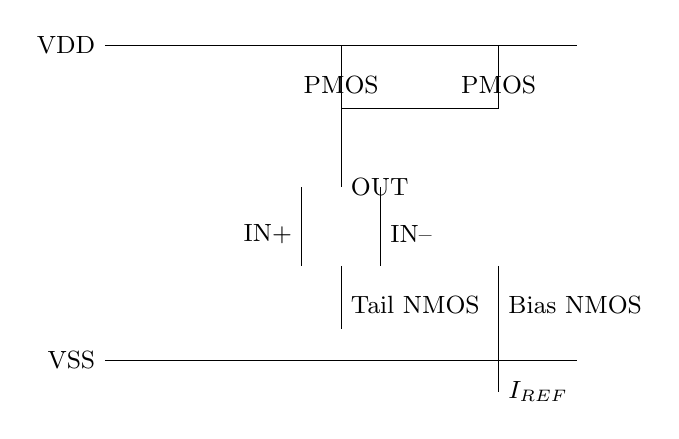
\begin{tikzpicture}[scale=1, every node/.style={font=\small}]
% Power rails
\draw (-1,4) node[left]{VDD} -- (5,4);
\draw (-1,0) node[left]{VSS} -- (5,0);

% PMOS mirror
\draw (2,4) -- (2,3.2);
\draw (4,4) -- (4,3.2);
\draw (2,3.2) -- (4,3.2);
\node at (2,3.5) {PMOS};
\node at (4,3.5) {PMOS};

% Output
\draw (2,3.2) -- (2,2.2);
\node[right] at (2,2.2) {OUT};

% NMOS diff pair
\draw (1.5,2.2) -- (1.5,1.2);
\draw (2.5,2.2) -- (2.5,1.2);
\node[left] at (1.5,1.6) {IN+};
\node[right] at (2.5,1.6) {IN--};

% Tail NMOS
\draw (2,1.2) -- (2,0.4);
\node[right] at (2,0.7) {Tail NMOS};

% Bias mirror
\draw (4,1.2) -- (4,0.4);
\node[right] at (4,0.7) {Bias NMOS};

% Reference current
\draw (4,0.4) -- (4,-0.4);
\node[right] at (4,-0.4) {$I_{REF}$};
\end{tikzpicture}
\end{center}

\section{Device Dimensions (Use Exactly These Values)}

All devices use standard-threshold 1.8 V transistors.

\subsection{NMOS Differential Pair (M1, M2)}
\begin{itemize}
  \item Device: \texttt{sky130\_fd\_pr\_\_nfet\_01v8}
  \item $W = 10\ \mu$m, $L = 1.0\ \mu$m
  \item Fingers: 2 $\times$ 5 $\mu$m
  \item Bulk: VSS
\end{itemize}

\subsection{PMOS Active Load (M3, M4)}
\begin{itemize}
  \item Device: \texttt{sky130\_fd\_pr\_\_pfet\_01v8}
  \item $W = 20\ \mu$m, $L = 1.0\ \mu$m
  \item Fingers: 4 $\times$ 5 $\mu$m
  \item Bulk: VDD
\end{itemize}

\subsection{Tail NMOS (Mirrored) (M5)}
\begin{itemize}
  \item Device: \texttt{sky130\_fd\_pr\_\_nfet\_01v8}
  \item $W = 8\ \mu$m, $L = 2.0\ \mu$m
  \item Bulk: VSS
\end{itemize}

\subsection{Bias NMOS (Reference Mirror) (M6)}
\begin{itemize}
  \item Device: \texttt{sky130\_fd\_pr\_\_nfet\_01v8}
  \item $W = 8\ \mu$m, $L = 2.0\ \mu$m
  \item Diode-connected
  \item Bulk: VSS
\end{itemize}

\section{Bias Conditions}

\begin{itemize}
  \item External reference current: $I_{REF} = 10\ \mu$A
  \item OTA tail current: $\approx 10\ \mu$A
  \item Per-branch current: $\approx 5\ \mu$A
\end{itemize}

\section{Target Performance (Typical)}

\begin{itemize}
  \item DC Gain: 20--35 dB
  \item Unity Gain Bandwidth: 1--3 MHz
  \item Power Consumption: $\sim$18 $\mu$W
  \item Output swing: $\sim$0.3--1.4 V
\end{itemize}

\section{Required Simulations}

\begin{itemize}
  \item Operating point (.op)
  \item DC transfer curve
  \item AC gain (.ac)
\end{itemize}

\section{Layout Rules}

\begin{itemize}
  \item Common-centroid differential pair
  \item Symmetric PMOS mirror
  \item Guard ring around OTA
  \item Explicit bulk connections
  \item Shared diffusions where possible
  \item Metal 5 is \textbf{prohibited} (reserved for TinyTapeout power grid)
  \item Use metal1--metal4 only for routing
\end{itemize}

\section{TinyTapeout Analog Pin Mapping}

\begin{itemize}
  \item \texttt{ua[0]}: VIN+ (positive differential input)
  \item \texttt{ua[1]}: VIN-- (negative differential input)
  \item \texttt{ua[2]}: VOUT (single-ended output)
  \item \texttt{ua[3]}: IREF (external 10$\mu$A reference current)
\end{itemize}

\section{3-Session Lesson Plan (2 Hours Each)}

\subsection*{Session 1: Schematic Design \& Simulation}
\textbf{Tools: xschem, ngspice}

\begin{itemize}
  \item OTA architecture overview
  \item Schematic entry using provided sizes
  \item External reference current setup
  \item Operating-point and AC simulation
\end{itemize}

\noindent\textbf{Deliverable:} Passing simulations (gain, bandwidth, operating point)

\subsection*{Session 2: Layout and DRC}
\textbf{Tools: Magic VLSI}

\begin{itemize}
  \item Analog layout principles
  \item Differential pair common-centroid layout
  \item PMOS mirror layout
  \item Guard rings and power routing
  \item DRC cleanup
\end{itemize}

\noindent\textbf{Deliverable:} DRC-clean layout

\subsection*{Session 3: LVS and Tapeout}
\textbf{Tools: netgen, Magic}

\begin{itemize}
  \item LVS debugging and fixes
  \item Optional parasitic extraction
  \item GDS export
  \item TinyTapeout submission
\end{itemize}

\noindent\textbf{Deliverable:} Final GDS submitted to TinyTapeout

\section{Final Note to Participants}

\begin{quote}
``If your OTA has gain and passes LVS, you have successfully taped out an analog IC.''
\end{quote}

\end{document}
